\chapter{Présentation générale}



%doit contenir la fonction de ce rapport : etat de l'art + previsionnel
%dans le but de réaliser un projet
\section{Présentation du projet}
Aujourd'hui, détecter les points des articulations du corps humain 
est une technique courante, grâce à certain périphérique tel que la 
Kinect. Les points des articulations du corps forment le squelette 3D. 
Cependant, les squelettes 3D sont en générales peu riche en informations 
concernant les points des articulations des mains.\\
 
Pourtant les mains sont habiles et nous pouvons faire de nombreux 
mouvements, plus ou moins complexes et rapides avec elles. De plus en 
plus d'application nécessite des IHM plus précisent et plus 
naturelles. Utiliser ces mains pour contrôler, interagir et communiquer 
avec un ordinateur, devient de plus en plus intéressant. Ce niveau de 
précision peut être utile dans divers domains :
\begin{itemize}
  \item simulation médicale.
  \item modélisation et CAO.
  \item manipulation d'objets 3D virtuels.
  \item jeux vidéo.\\
\end{itemize}

Le projet \og Hand Kinect \fg consiste à extraire depuis une Kinect 2, 
les points correspondants aux articulations du corps grâce aux 
fonctions du SDK de Kinect. De plus, nous devons récupérer les points 
des articulations des mains, nous disposons d'un module fourni par 
nos tuteurs de projet. Ainsi, l'assemblage de ces points nous permet 
d'obtenir le squelette 3D complet de la personne devant la Kinect.\\

\begin{figure}[H]
  \begin{center}
    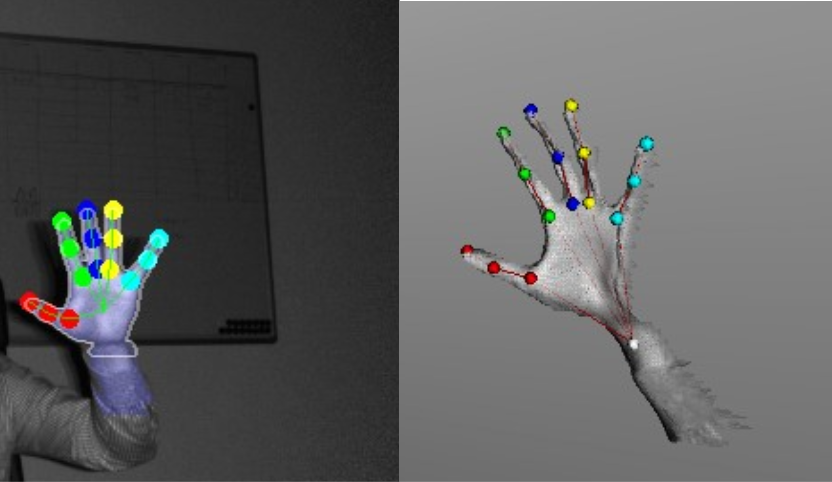
\includegraphics[width=350px]{images/joint_detection.png}
    \caption{Détection des articulations des mains}
  \end{center}
\end{figure}

Ensuite, nous souhaitons animer un modèle 3D, qui peut être un modèle 
d'humain, de robot ou bien de créature. Les mouvement de ce modèle 
doivent suivre les points du squelette préalablement détecté, de 
manière cohérente par rapport au mouvement de la personne devant la 
Kinect. Nous utilisons Unity3D, pour cette partie de 
modélisation.\\

Unity3D est un moteur de jeu qui permet de développé rapidement des 
environnement et application 3D. Il est facile d'obtenir des 
application compatible sur de nombreuse plateforme. Ce moteur 
propose également une licence gratuit accés compléte.\\

\begin{figure}[H]
  \begin{center}
    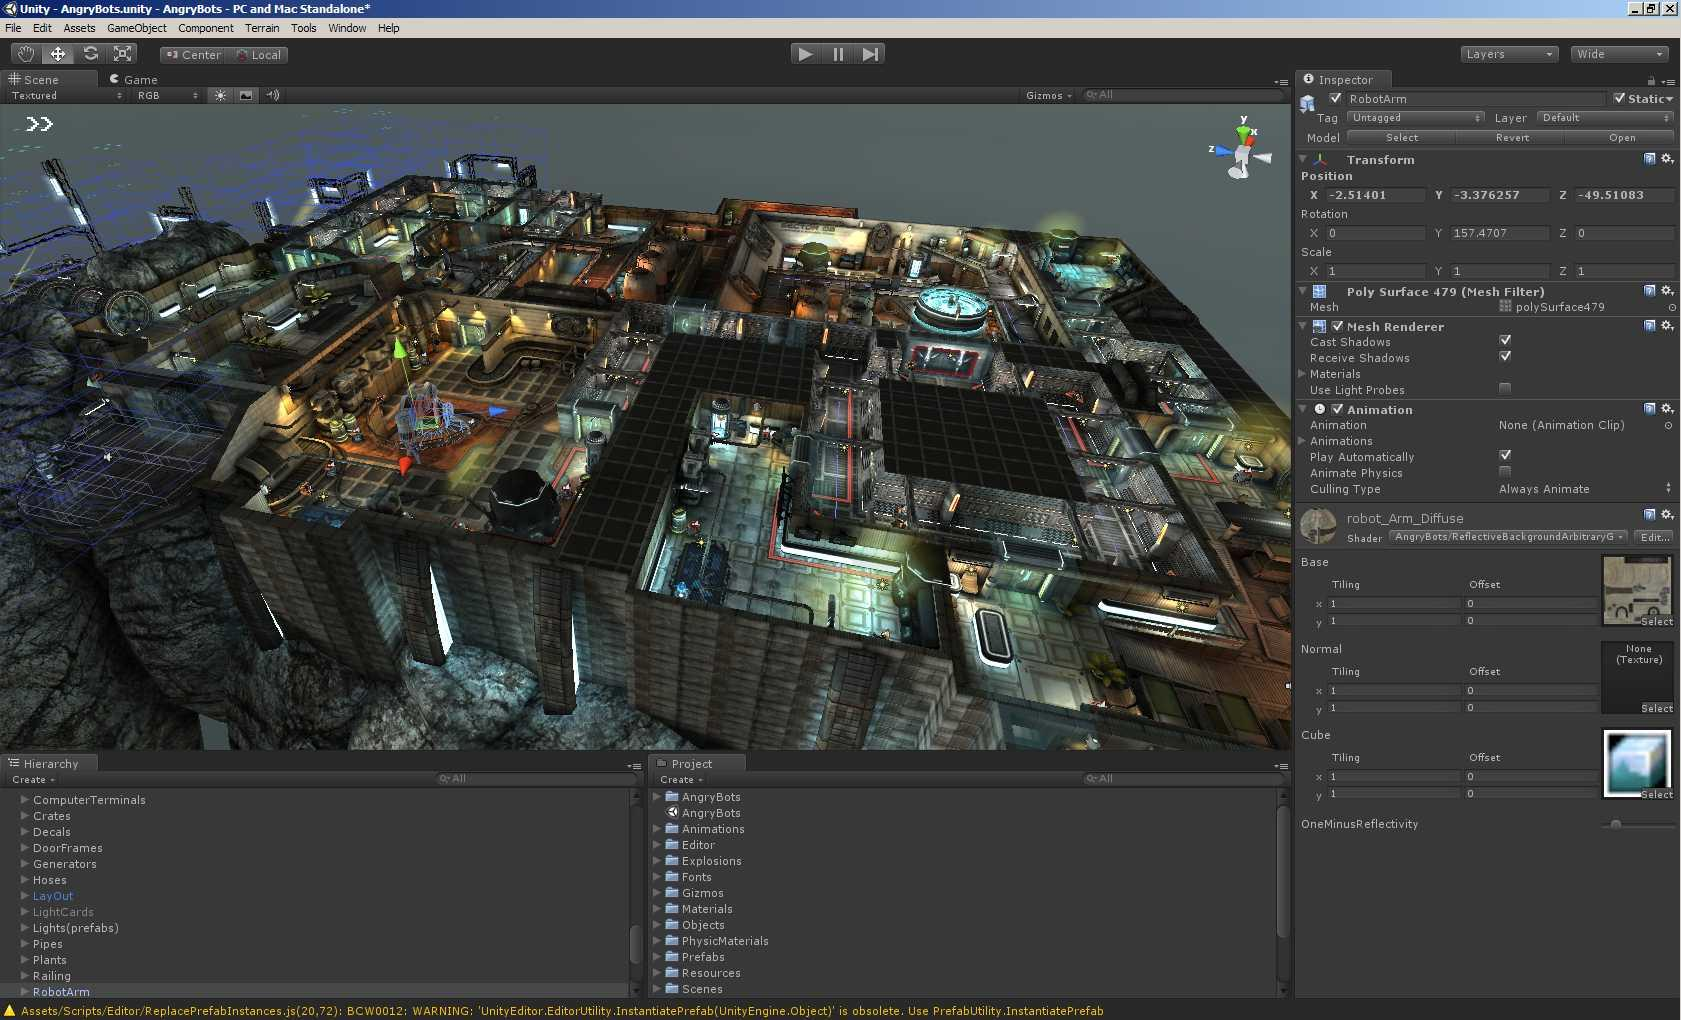
\includegraphics[width=350px]{images/Unity3D.jpg}
    \caption{Interface de Unity3D}
  \end{center}
\end{figure}

Dans le cadre de ce projet, nous sommes amené à rédiger un état de la 
l'art. Cette première partie, nous permet de synthétiser et sélectionner 
les solutions. Notre objectif étant de détecter la main et les 
articulations de la main d'une personne, afin de modéliser en 3D la main 
de cette personne, dans des plans de caméra global ou rapprocher. Cela 
doit être réalisable en temps réel et à partir d'une caméra nous 
fournissant une image RGB et une image contenant l'information de 
profondeur de la scène filmée.\\

%doit contenir l'ensemble des informations sur l'équipe -> sur quoi porte leur recherche
\section{Contexte}
La réalisation de ce projet se fait avec l'équipe 3D 
SAM\footnote{Modeling and Analysis of Static and Dynamic Shapes}. 
Cette équipe appartient au centre CRIStAL\footnote{Centre de Recherche 
en Informatique, Signal et Automatique de Lille}. Ce centre de 
recherche est le nouveau pôle de recherche qui regroupe les 
laboratoires d'Informatique, Signal et Automatique de Lille.\\


L'équipe 3D SAM est basée à l'école d'ingénieur Télécom Lille 1. 
Cette équipe conçoit de nouveaux outils et méthodes d'analyse des 
formes des objets 3D statiques et dynamique. Ils travaillent sur 
l'analyse de formes des objects 3D et la modélisation des variations 
des formes dans des vidéos 3D.

\begin{figure}[H]
  \begin{center}
    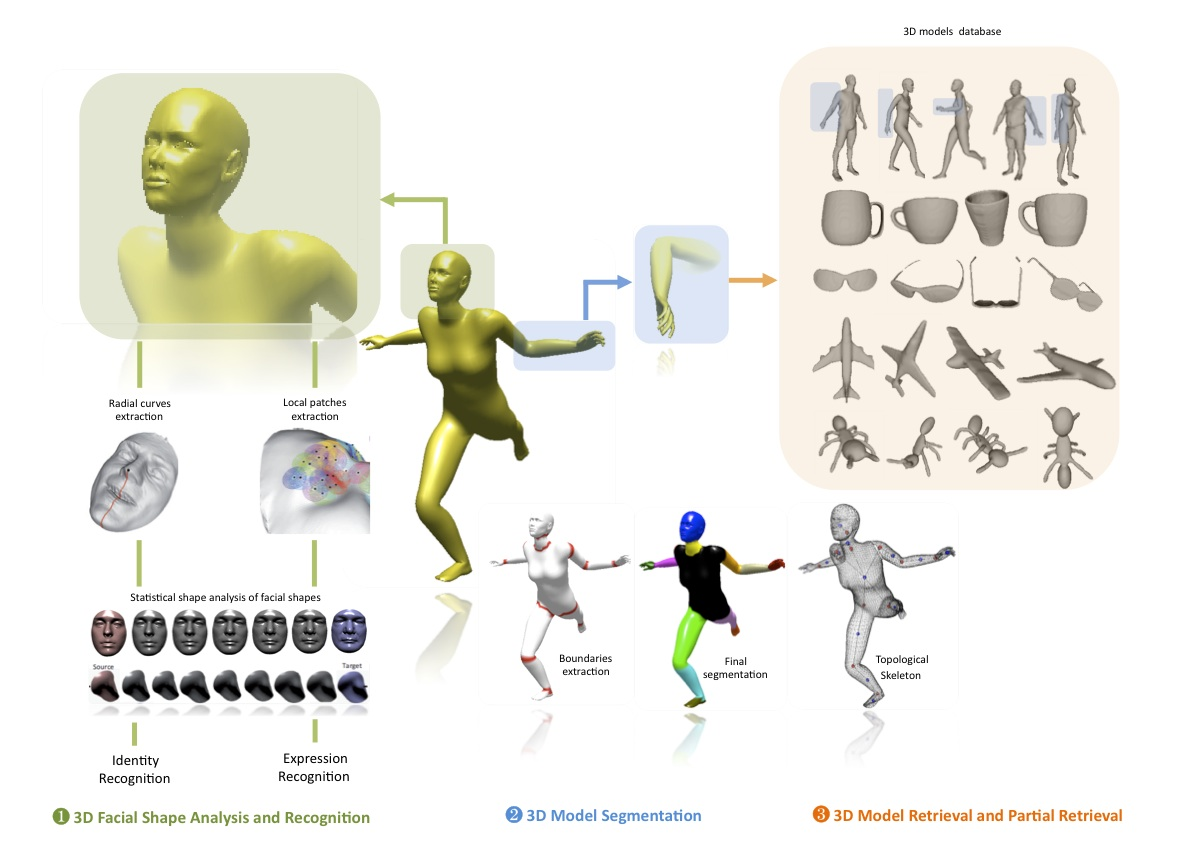
\includegraphics[width=300px]{images/accueil-illus.jpg}
    \caption{Exemples de travaux de l'équipe 3D SAM}
  \end{center}
\end{figure}

Le projet \og Hand Kinect \fg est un nouveau projet proposé par 
l'équipe. Nous sommes les premiers à travailler sur ce projet, il 
ne s'agit pas d'une reprise d'un projet déjà entamé auparavant.\\

Pour la réalisation de ce projet, nous disposons d'une caméra Kinect2. 
Pour les représentation et animation 3D, il nous faut un environnement 
de modélisation 3D, nous utilisons Unity3D comme montré précédemment. 
Nous disposons également, d'un module nous permettant d'extraire les 
points des articulation de la main.

%pourquoi faire ce projet (plus de precision?) + cas concret ou on pourrait l'utiliser (ex : medecine)
\section{Problèmatique}
D'abord, la Kinect 2 peux déjà de suivre 6 personne à la fois. Elle 
détecte un squelette de 25 points (voir Fig. 
\ref{fig:skeleton_kinect2}). Cependant, les mains ne sont représentées 
que par 3 point, qui sont le centre de main, le pouce et le bout du 
majeur. C'est une amélioration par rapport à la Kinect 1, qui de 
détecter que le centre de la main.\\

%a revoir
D'autre outils permettent de détecter les mains des utilisateurs. Par exemple le Leap Motion détecte les articulations des mains. Néanmoins,
ce capteur est limité car il faut garder les mains proches et dans le 
cadre du capture. Leap Motion ne permet pas de détecter le squelette 
d'une personne.\\

%a revoir
À partir de ces constats nous pouvons formuler la problèmatique 
suivante. Puisque, 
les mains sont très habile, il peut être difficile de detecter de leurs 
articulations dans des positions contraignante. Autres choses, les 
problèmes liés à la luminausitée sont récurrents, il est souhaitable 
d'utiliser des techniques robustent et invariantent à la luminausitée, 
mais qui restent efficace. De plus, il existe encore peu de méthodes 
permettant de détecter la pose et les articulations des mains dans 
un point de vue de caméra qui permetterais de retrouver l'ensemble du
squelette humain.  

%comment réaliser ce projet, avec quoi + résultat attendu
\section{Objectif}
L'objectif de notre projet est d'utiliser la Kinect 2 dans le but de détecter les différentes articulations
de la main et de modéliser celle-ci dans une application Unity.
%TODO ajouter les différentes étape de nos recherches 

\section{Présentation de la Kinect 2}
La Kinect 2 de Microsoft possède une caméra couleur en mode YUV de 1920x1080 pixel.
YUV est une combination particulière d'information pour restituer la couleur, comme RGB ou HSP.
Cette combinaison aussi appelée YCbCr, avec Y la luminance, U/Cb la composante bleu sans luminance et V/Cr la composante rouge sans luminance
En plus de sa caméra, elle possède 3 diffuseur de rayonnement infrarouges qui servent à dessiner une carte de profondeur.
Les autres fonctionnalités ne nous intéresseront pas résoudre notre problèmatique.\\

\begin{figure}[H]
 \center
 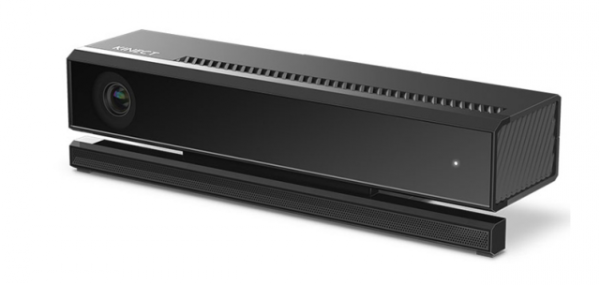
\includegraphics[width=300px]{images/kinect-v2.png}
 \caption{Caméra Kinect 2}
\end{figure}

On récupère donc de Kinect les données brutes suivantes : 
\begin{itemize}
 \item un flux vidéo couleur en YUV
 \item un flux vidéo d'images de profondeur
\end{itemize}

Ces deux flux peuvent servir à détecter la main (méthodes expliquées dans la partie état de l'art).
Le SDK de la Kinect fournit des informations déjà traitées. 
Par exemple pour notre projet, les jointures du poignet, du centre de la main, du sommet du pouce et du sommet du majeur.

\begin{figure}[H]
\center
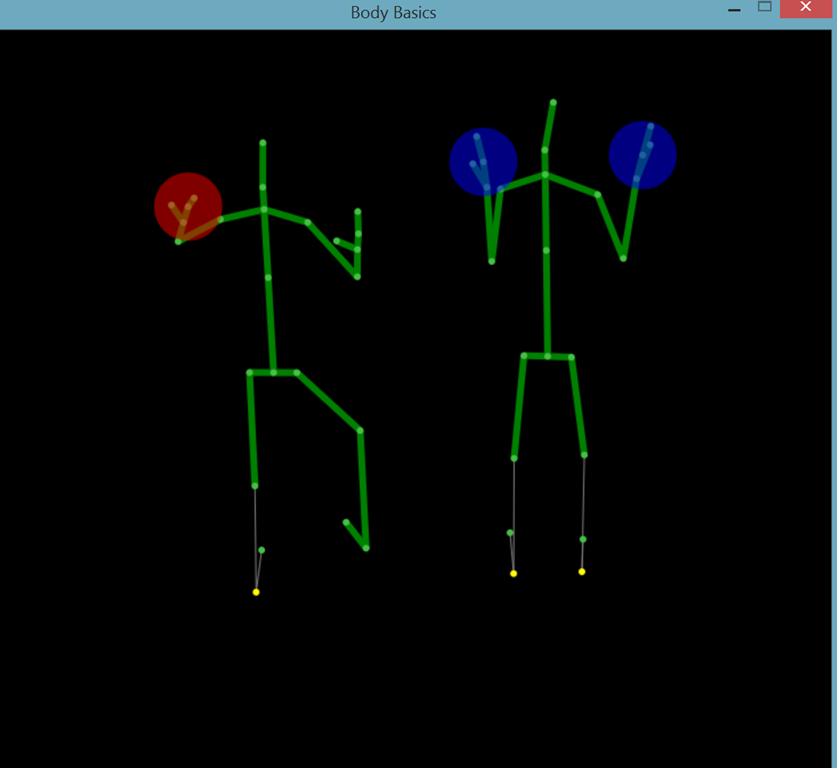
\includegraphics[width=250px]{images/kinec2_skel.png}
\caption{Squelette de l'utilisateur détecté par la Kinect 2}
\label{fig:skeleton_kinect2}
\end{figure}

%présentation du materiel + image materiel
%présentation des données brut
%présentation du sdk + image squelette
